% Options for packages loaded elsewhere
\PassOptionsToPackage{unicode}{hyperref}
\PassOptionsToPackage{hyphens}{url}
%
\documentclass[
  12pt,
]{article}
\usepackage{lmodern}
\usepackage{amsmath}
\usepackage{ifxetex,ifluatex}
\ifnum 0\ifxetex 1\fi\ifluatex 1\fi=0 % if pdftex
  \usepackage[T1]{fontenc}
  \usepackage[utf8]{inputenc}
  \usepackage{textcomp} % provide euro and other symbols
  \usepackage{amssymb}
\else % if luatex or xetex
  \usepackage{unicode-math}
  \defaultfontfeatures{Scale=MatchLowercase}
  \defaultfontfeatures[\rmfamily]{Ligatures=TeX,Scale=1}
  \setmainfont[]{Times New Roman}
\fi
% Use upquote if available, for straight quotes in verbatim environments
\IfFileExists{upquote.sty}{\usepackage{upquote}}{}
\IfFileExists{microtype.sty}{% use microtype if available
  \usepackage[]{microtype}
  \UseMicrotypeSet[protrusion]{basicmath} % disable protrusion for tt fonts
}{}
\makeatletter
\@ifundefined{KOMAClassName}{% if non-KOMA class
  \IfFileExists{parskip.sty}{%
    \usepackage{parskip}
  }{% else
    \setlength{\parindent}{0pt}
    \setlength{\parskip}{6pt plus 2pt minus 1pt}}
}{% if KOMA class
  \KOMAoptions{parskip=half}}
\makeatother
\usepackage{xcolor}
\IfFileExists{xurl.sty}{\usepackage{xurl}}{} % add URL line breaks if available
\IfFileExists{bookmark.sty}{\usepackage{bookmark}}{\usepackage{hyperref}}
\hypersetup{
  pdftitle={What's the Catch? Recreational Fishing Trends in North Carolina (1990-2019)},
  pdfauthor={Ardath Dixon, Annie Harshbarger, Eva May},
  hidelinks,
  pdfcreator={LaTeX via pandoc}}
\urlstyle{same} % disable monospaced font for URLs
\usepackage[margin=2.54cm]{geometry}
\usepackage{graphicx}
\makeatletter
\def\maxwidth{\ifdim\Gin@nat@width>\linewidth\linewidth\else\Gin@nat@width\fi}
\def\maxheight{\ifdim\Gin@nat@height>\textheight\textheight\else\Gin@nat@height\fi}
\makeatother
% Scale images if necessary, so that they will not overflow the page
% margins by default, and it is still possible to overwrite the defaults
% using explicit options in \includegraphics[width, height, ...]{}
\setkeys{Gin}{width=\maxwidth,height=\maxheight,keepaspectratio}
% Set default figure placement to htbp
\makeatletter
\def\fps@figure{htbp}
\makeatother
\setlength{\emergencystretch}{3em} % prevent overfull lines
\providecommand{\tightlist}{%
  \setlength{\itemsep}{0pt}\setlength{\parskip}{0pt}}
\setcounter{secnumdepth}{5}
\usepackage{booktabs}
\usepackage{longtable}
\usepackage{array}
\usepackage{multirow}
\usepackage{wrapfig}
\usepackage{float}
\usepackage{colortbl}
\usepackage{pdflscape}
\usepackage{tabu}
\usepackage{threeparttable}
\usepackage{threeparttablex}
\usepackage[normalem]{ulem}
\usepackage{makecell}
\usepackage{xcolor}
\ifluatex
  \usepackage{selnolig}  % disable illegal ligatures
\fi

\title{What's the Catch? Recreational Fishing Trends in North Carolina
(1990-2019)}
\usepackage{etoolbox}
\makeatletter
\providecommand{\subtitle}[1]{% add subtitle to \maketitle
  \apptocmd{\@title}{\par {\large #1 \par}}{}{}
}
\makeatother
\subtitle{\url{https://github.com/ardathdixon/Data_FinalProject}}
\author{Ardath Dixon, Annie Harshbarger, Eva May}
\date{Spring 2021}

\begin{document}
\maketitle

\newpage
\tableofcontents 
\newpage
\listoftables 
\newpage
\listoffigures 
\newpage

\hypertarget{rationale-and-research-questions}{%
\section{Rationale and Research
Questions}\label{rationale-and-research-questions}}

As public awareness of increasing strains on ocean resources and
organisms grows (e.g.~see the reach of films such as Seaspiracy and
Sonic Sea), more attention is being placed on understanding fishing
patterns and the impacts they have on the oceans. Most of this attention
is placed on commercial and industrial fishing operations, which are
studied and managed by the federal agency NOAA, the National Oceanic and
Atmospheric Administration. However, there are fewer studies on
recreational fishing, for which NOAA also collects data and aids in
overseeing.

For this study, we chose to investigate recreational fishing trends in
North Carolina over a thirty-year period. The data, whose origins are
discussed more below, initially included 27 variables, detailing
information such as mode of fishing and wave (2-month time period) in
which the fish were caught. For this analysis, we wanted to look
specifically at total catch during each wave, as we were running time
series analyses during the course of the project. Therefore, we focused
on only one catch estimation variable: total catch. We chose North
Carolina due to our familiarity with species here, and we chose two
popular recreational fishing species to investigate alongside all
species combined. Trends in recreational fishing data can give us
information about human behavior, species populations, and species
movement patterns, which is why we found this topic interesting and
wanted to investigate it further.

We chose the following questions to guide our work:

\begin{enumerate}
\def\labelenumi{\arabic{enumi}.}
\item
  Are there trends in the amount of these fish caught over time? How do
  they compare?
\item
  What could these trends look like in the future?
\end{enumerate}

\newpage

\hypertarget{dataset-information}{%
\section{Dataset Information}\label{dataset-information}}

\hypertarget{data-retrieval}{%
\subsection{Data Retrieval:}\label{data-retrieval}}

For this analysis, we used data collected during Marine Recreational
Information Program (MRIP) surveys conducted by NOAA
(\href{https://www.fisheries.noaa.gov/recreational-fishing-data/about-marine-recreational-information-program}{\textbf{NOAA
n.d.}}). NOAA works with state and local partners to collect information
on the species and number of fish caught by fishers via in-person
communication, telephone surveys, and mail-in surveys. We retrieved the
data using the NOAA Recreational Fisheries Statistics Queries ``download
query'' tool (found
\href{https://www.fisheries.noaa.gov/data-tools/recreational-fisheries-statistics-queries}{\textbf{here}}).
We created three separate queries to download data: one for all species,
one for bluefish (\emph{Pomatomus saltatrix}), and one for black sea
bass (\emph{Centropristis striata}). For each query, we used the date
range 1990-2019 and requested catch estimate data by ``wave'', or
two-month period, for all waves, fishing modes, and areas of fishing for
the state of North Carolina (Table 1). We downloaded the CSVs as ZIP
files and added them to our project repository. All data and code for
this project can be retrieved from the
\href{https://github.com/ardathdixon/Data_FinalProject}{\textbf{GitHub
repository}}.

\begin{table}[H]

\caption{\label{tab:table1}General Information About the Data Used}
\centering
\begin{tabular}[t]{l|>{\raggedright\arraybackslash}p{5in}}
\hline
Detail & Description\\
\hline
Data Source & NOAA MRIP\\
\hline
Retrieved from & https://www.fisheries.noaa.gov/data-tools/recreational-fisheries-statistics-queries\\
\hline
Variables Used & Year, Wave, Total Catch (Number of fish), Mode, Area\\
\hline
Date Range & January 1990 - December 2019\\
\hline
\end{tabular}
\end{table}

\hypertarget{data-wrangling}{%
\subsection{Data Wrangling:}\label{data-wrangling}}

We began our analysis by selecting the following columns from the raw
data CSV files: Year, Wave, Mode, Area, and Total Catch. Next, we
created a custom function to convert waves to months in order to process
the six annual waves using time series analysis. For NOAA fishing
records, wave 1 represents January and February, wave 2 represents March
and April, and this continues through the year. Therefore, we assigned
wave 1 catches to the date of January 1, wave 2 catches to March 1, and
so forth.

After applying the custom wave-to-month function to the data, we created
a date variable to capture year and month together (the day value for
each of these dates was 01). Next, we used a split-apply-combine
approach to find the sum of total catch for each wave. Each of these
sums contains the catch from all unique combinations of fishing mode and
area that were recorded during a given wave. Finally, to create the time
series, we selected only the columns for date (DATE) and the sum of
total catch (TOT\_CAT\_ALL). We computed summary statistics for these
total catch values, as shown in Table 2. We then proceeded with
exploratory analysis and interpolation of missing data points, which are
described below.

\begin{table}[H]

\caption{\label{tab:table2}Total Catch Summaries (Number of Fish)}
\centering
\begin{tabular}[t]{l|r|r|r}
\hline
Summary Statistic & All Fish & Bluefish & Black Sea Bass\\
\hline
Minimum & 11869 & 26 & 1168\\
\hline
Mean & 12402954 & 1342064 & 411196\\
\hline
Median & 11292146 & 1064369 & 313437\\
\hline
Maximum & 34932698 & 5254124 & 1746847\\
\hline
\end{tabular}
\end{table}
\newpage

\hypertarget{exploratory-analysis}{%
\section{Exploratory Analysis}\label{exploratory-analysis}}

Following initial wrangling, we checked the number of waves without
catch records for each dataset by joining the existing data to a list of
all possible waves between wave 1 of 1990 (represented by 1990-01-01)
and wave 6 of 2019 (represented by 2019-11-01). The results of this
exploration, which informed our approach for interpolation, can be found
in Table 3.

\begin{table}[H]

\caption{\label{tab:table3}Number of missing values from NOAA MRIP data}
\centering
\begin{tabular}[t]{l|r}
\hline
Dataset & Number of missing values\\
\hline
All fish & 11\\
\hline
Bluefish & 17\\
\hline
Black sea bass & 13\\
\hline
\end{tabular}
\end{table}

There were relatively few missing catch totals, and no more than one
consecutive data point was missing in a row. To fill the gaps with no
data, we used linear interpolation to estimate the likely values of
missing time periods. This interpolation incorporated the catch numbers
on either side of the missing value chronologically. If wave 1 of 1990
or wave 6 of 2019 was missing, we did not interpolate the value, as
there would not be a measurement available on both sides. We graphed the
total catch trends over time (with the newly interpolated values for
missing periods) as shown in Figure 1. With this visualization, we could
compare the three categories' recreational fishing catch patterns: all
fish, bluefish, and black sea bass.

\begin{figure}[H]

\hfill{}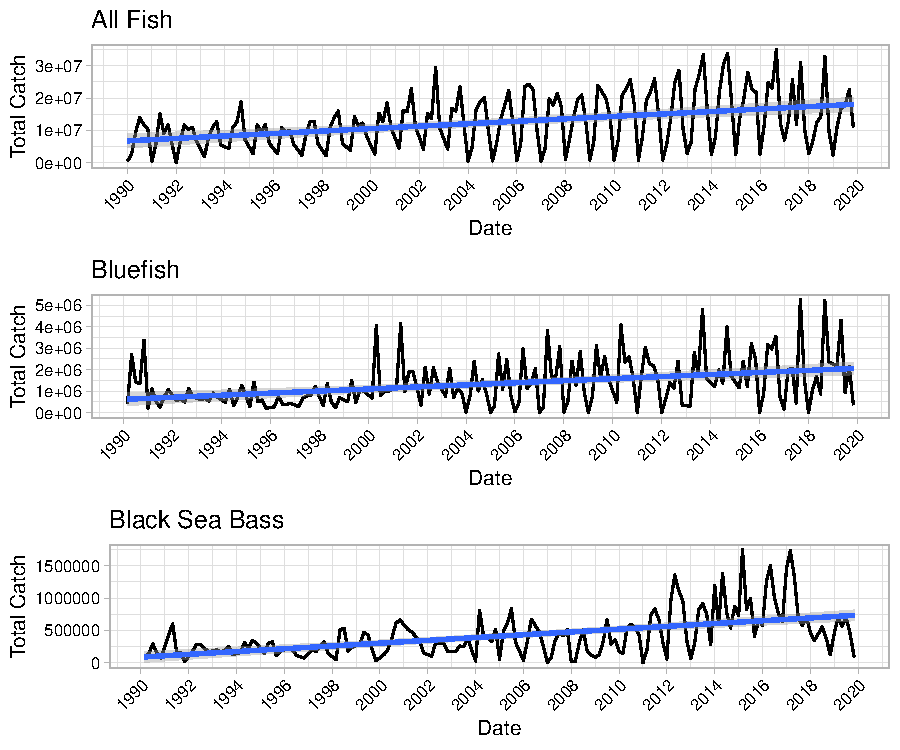
\includegraphics{Report_FishTrends_files/figure-latex/ggplot-1} 

\caption{Total Catch Patterns over Time}\label{fig:ggplot}
\end{figure}

\newpage

\hypertarget{analysis}{%
\section{Analysis}\label{analysis}}

\hypertarget{question-1-are-there-trends-in-the-amount-of-these-fish-caught-over-time-how-do-they-compare}{%
\subsection{Question 1: Are there trends in the amount of these fish
caught over time? How do they
compare?}\label{question-1-are-there-trends-in-the-amount-of-these-fish-caught-over-time-how-do-they-compare}}

After our interpolation of the missing data points for each dataset and
exploratory analysis, we created three time series for further analysis.
We investigated the trends in total catch for all fish (Figure 2),
bluefish (Figure 3), and black sea bass (Figure 4) by decomposing the
time series into their seasonal, trend, and remainder components. For
all three time series, we observed a strong seasonal trend with low
catch totals in the winter and high catch totals in the summer.
Furthermore, each trend component showed an apparent increase in total
catch over time.

Though all three datasets show an increasing trend over time, the
magnitude of this increase varies. The trend component of the time
series has a range of 12,667,496 for all fish, 2,237,223.2 for bluefish,
and 1,115,112.3 for black sea bass. The IQR for the trend component of
the time series was 5,528,819 for all fish, 976,185 for bluefish, and
245,287 for black sea bass.

\begin{figure}[H]

\hfill{}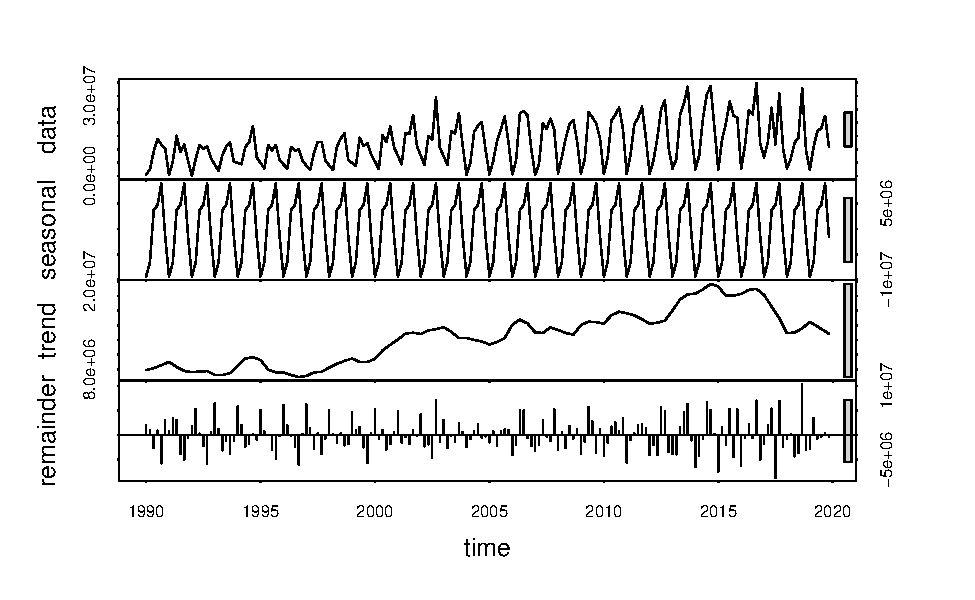
\includegraphics{Report_FishTrends_files/figure-latex/All Fish Trends-1} 

\caption{Seasonal and Trend Decomposition for All Fish Total Catch}\label{fig:All Fish Trends}
\end{figure}

\begin{figure}[H]

\hfill{}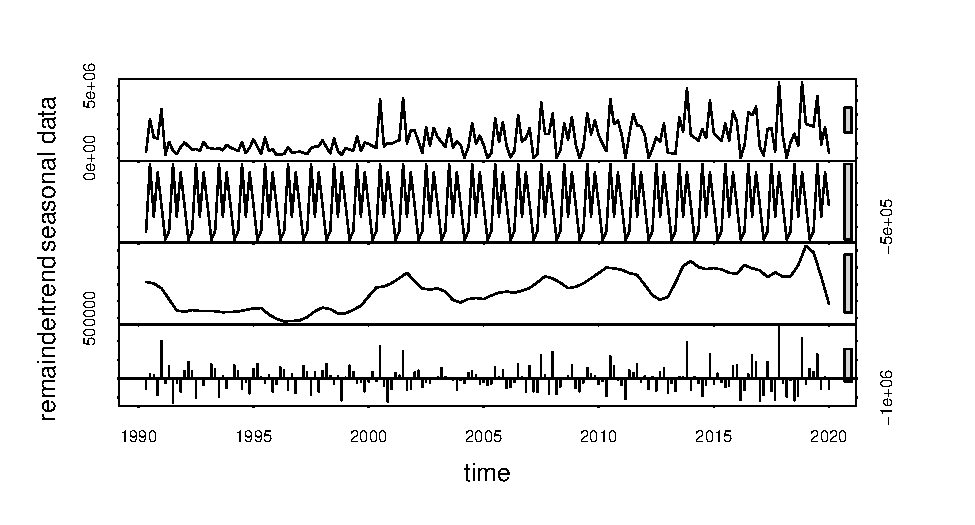
\includegraphics{Report_FishTrends_files/figure-latex/Bluefish Trends-1} 

\caption{Seasonal and Trend Decomposition for Bluefish Total Catch}\label{fig:Bluefish Trends}
\end{figure}

\begin{figure}[H]

\hfill{}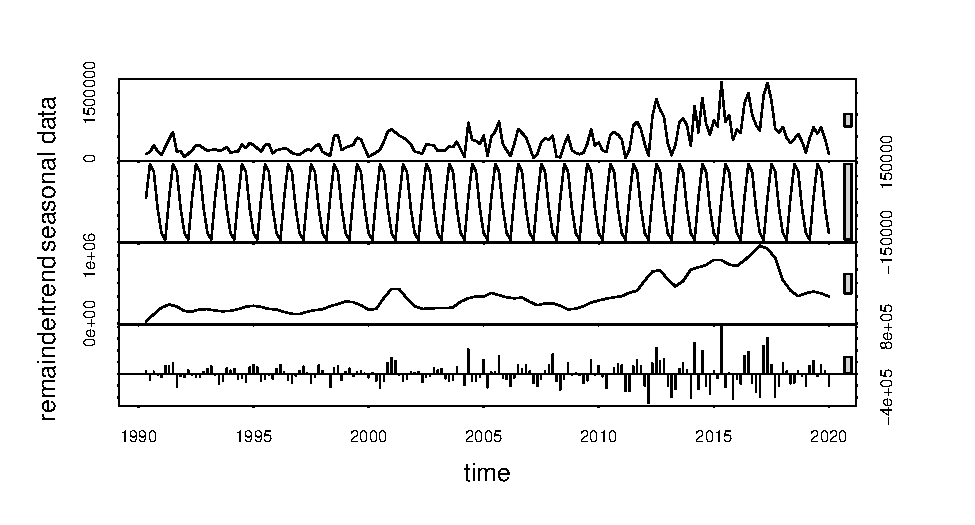
\includegraphics{Report_FishTrends_files/figure-latex/Black Sea Bass Trends-1} 

\caption{Seasonal and Trend Decomposition for Black Sea Bass Total Catch}\label{fig:Black Sea Bass Trends}
\end{figure}

We ran a Seasonal Mann-Kendall test on each time series to test whether
there was a monotonic trend in the total number of fish caught over time
(Table 4). All three tests returned a statistically significant result
(all fish: tau = 0.49, p \textless{} 2.22 x 10\^{}-16; bluefish: tau =
0.32, p = 8.75 x 10\^{}-10; black sea bass: tau = 0.41, p = 8.44 x
10\^{}-15). Therefore, for all three time series, we reject the null
hypothesis that there is no monotonic trend in favor of the alternative
hypothesis that there is a trend in the data over time.

\begin{table}[H]

\caption{\label{tab:table4}Seasonal Mann Kendall Tests}
\centering
\begin{tabular}[t]{l|r|l}
\hline
Fish Category & tau & 2-Sided P-value\\
\hline
All Fish & 0.4896552 & 0.000000e+00\\
\hline
Bluefish & 0.3235180 & 8.748902e-10\\
\hline
Black Sea Bass & 0.4095312 & 8.437695e-15\\
\hline
\end{tabular}
\end{table}

\emph{Note on Table 4: p-values in this table were generated from
wrangling the outputs from the seasonal Mann-Kendall tests. This
wrangling rounded the p-value for all fish from \textless{} 2.22 x
10\^{}-16 to 0.}

The strengths of these trends vary; based on tau values, catch for all
fish has the strongest overall trend while bluefish has the weakest
overall trend. Nonetheless, total catch for both individual species and
all species combined increases between the beginning of 1990 and the end
of 2019.

\hypertarget{question-2-what-could-these-trends-look-like-in-the-future}{%
\subsection{Question 2: What could these trends look like in the
future?}\label{question-2-what-could-these-trends-look-like-in-the-future}}

To investigate future trends, we used forecasting in R to predict future
data based on the existing past data we pulled from NOAA. There are
several different methods through which to forecast, though only some of
them account for seasonality, which was necessary here due to the
seasonal components found in all three of our time series. We chose to
use the Holt-Winters forecasting method for this data. Holt-Winters is
more complex than simpler methods like naive forecasting, but it
requires knowledge of fewer additional input variables that other
models, like SARIMA, need in order to run. Holt-Winters uses smooth
exponentiating and varying weights of past data - with more recent data
weighed more - to predict future data. Here, we predicted five years of
data (where h = number of periods, and each period = two months). In the
resulting plots, the dark blue area represents the 80\% confidence
interval level for predicted data, while the light blue area represents
the 95\% confidence interval level.

\begin{figure}[H]

\hfill{}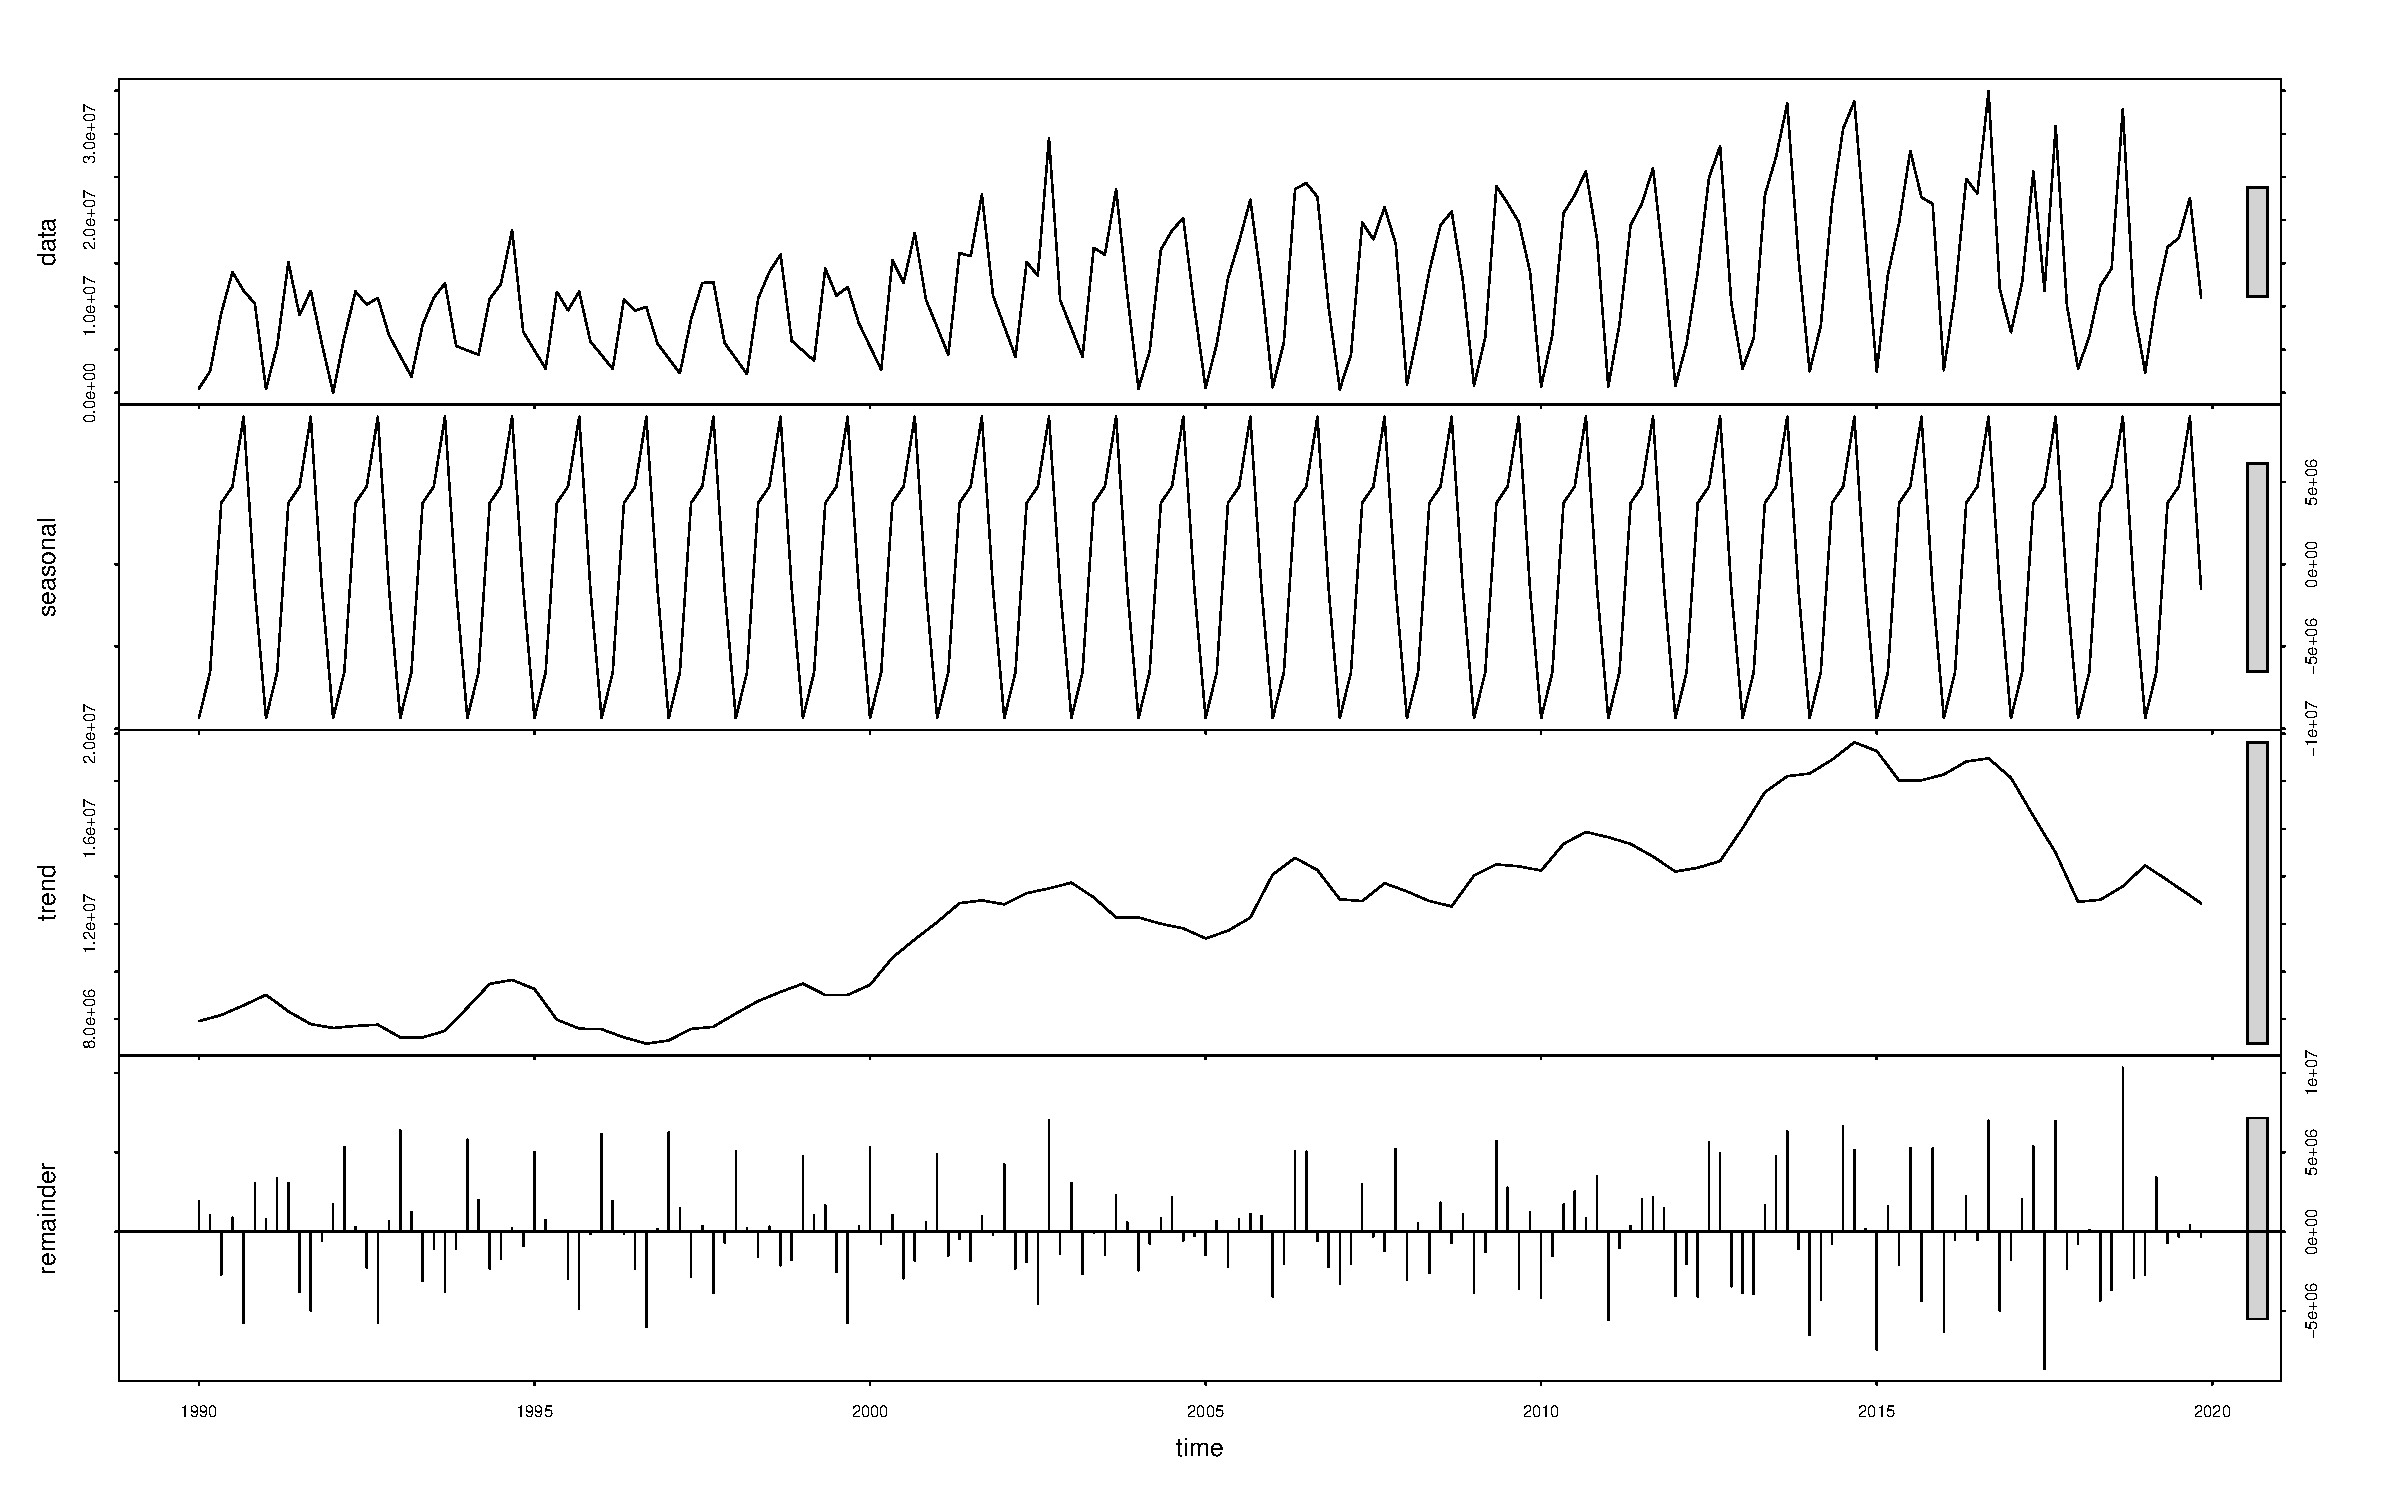
\includegraphics{Report_FishTrends_files/figure-latex/unnamed-chunk-1-1} 

\caption{Holt-Winters Catch Forecasts}\label{fig:unnamed-chunk-1}
\end{figure}

The Holt-Winters plots (Figure 5) all show clear continued seasonal
patterns and trends. For black sea bass and all species combined,
overall future trends are expected to be positive, like the past trends.
For bluefish, the forecasted trend is slightly negative -- this is
likely because the most recent years of bluefish data do show a slight
negative slope, even though the trend is positive for the full thirty
years in the dataset (though as noted above, bluefish has the smallest
tau, and therefore the weakest trend). These forecasting plots are
useful visualizations but should not be considered fully accurate
because of the inherent complexities in fishing catch data that models
like Holt-Winters cannot account for.

\newpage

\hypertarget{summary-and-conclusions}{%
\section{Summary and Conclusions}\label{summary-and-conclusions}}

\hypertarget{strong-seasonal-trends}{%
\subsection{Strong seasonal trends}\label{strong-seasonal-trends}}

NOAA marine recreational fishing catch totals for North Carolina show
strong seasonal trends. Many more fish are caught in the summer, and
much fewer fish are caught in the winter, as demonstrated above (Figure
1). This seasonality is likely influenced by recreational fishing
patterns, where fishers are more likely to fish in warm summer weather
than cool winter weather. Another potential cause for the seasonal
trends is fish abundance and migration patterns, with higher populations
of fish in North Carolina waters during the summer than during the
winter. Total catch trends for all fish and black sea bass showed
unimodal peaks and valleys overall, while bluefish showed bimodal trends
(Figure 1). These bimodal bluefish peaks could be due to their seasonal
migration patterns (\href{http://www.asmfc.org/species/bluefish}{ASMFC
2021}). Another possible explanation for their bimodal trends is that
bluefish in the northern Atlantic Ocean spawn twice annually, once in
the spring and once in the summer, and more fish may be caught during
spawning aggregations (Arthur \& Walford 1979).

\hypertarget{overall-positive-trend}{%
\subsection{Overall positive trend}\label{overall-positive-trend}}

There was an increase in total catch of bluefish, black sea bass, and
all species combined over time. The main driver of this increase in
recreational fishery landings is unknown, but it could be attributed to
increased fishing effort, with either more fishers participating in
recreational fishing or individual fishers catching more fish.

Although the trend was generally positive for all three time series, it
was not uniform; in other words, the rate of change varied over time,
and there were brief periods where catch plateaued or decreased. This
variation could be caused by changes in recreational fishing regulations
over time, such as the increase or decrease of catch limits and size
limits, or temporary area closures. Furthermore, recreational fishing is
subject to the myriad of factors that can influence human behavior,
including but not limited to climate variation (Dundas \& von Haefen
2020) and events with an environmental impact such as hurricanes (Smee
et al.~2020) or the Deepwater Horizon Oil Spill (Alvarez et al.~2014).
In a recent example of how other current events could impact
recreational fishing, the COVID-19 pandemic could have either increased
recreational fishing in 2020, when people were spending more time
outside, or decreased recreational fishing, as people were less able to
travel to the coast. This example is beyond the scope of our analysis,
which extends only to the end of 2019, but it demonstrates the
complexity of understanding and predicting patterns in recreational
fishing.

\hypertarget{limitations}{%
\subsection{Limitations}\label{limitations}}

The MRIP system works very well for its intended purposes, but it is
ultimately still a system based on estimation. Through MRIP, NOAA
interviews only some fishers, then uses mathematical modeling to
extrapolate on this collected survey data in order to create statewide
(or area-wide, depending on the dataset) estimates. While MRIP is the
best source of recreational fishing catch data, there is always room for
some error in its estimations.

Within each of our datasets, there were some missing values. These
values were not side by side or frequent, so we chose to linearly
interpolate our data in order to fill them in. This helped our figures
and analyses (e.g.~seasonal Mann-Kendall) to appear and run cleaner, but
interpolating has some drawbacks. While interpolations seemed to follow
the clear seasonal pattern in each dataset, most often the interpolated
data was in wave periods that were minimums in other years, so our
interpolated values may have been a bit higher than actual catch rates
during those times. Interpolation is an estimator for missing data, and
it is important to acknowledge that our interpolated data may not be
representative of true values.

Finally, our forecasted data was much cleaner and less noisy than our
existing data (see Figure 5). Noise in these datasets comes from
external factors like changes in fish catch limits or weather patterns,
which this forecasting method can neither take into account nor predict.
Our forecasting outputs were therefore limited by the relatively simple
methodology we chose to employ. Holt-Winters remains a popular
forecasting method and is reasonable to use for our purposes here, but
the inherent uncertainty in this predicted data is also important to
acknowledge.

\hypertarget{future-recommendations}{%
\subsection{Future recommendations}\label{future-recommendations}}

Future research could extend our analysis to include a greater scope
regarding specific species, areas, and timelines. NOAA provides catch
data for an extensive number of fish species, and therefore time-series
and forecasting analyses could also be applied to other species of
interest. Likewise, the widespread area available for NOAA catch data
means that future research could translate our analysis toward catch
numbers from other states. Additionally, the available data goes beyond
the timeline we analyzed, dating back to 1981. Future analysis could
adjust variables of interest accordingly thanks to the vast
\href{https://www.fisheries.noaa.gov/data-tools/recreational-fisheries-statistics-queries}{NOAA
data available for public access}.

In addition to adjusting the sample for analysis, future research could
compare changes of catch per unit of effort over time. Analyzing total
catch does not incorporate the number of fishers or success rates.
Incorporating the catch per unit of effort could reveal possible causes
of the increasing catch trends over time (e.g.~more fishers in total or
more efficient fishers).

\newpage

\hypertarget{references}{%
\section{References}\label{references}}

Alvarez, S., Larkin, S. L., Whitehead, J. C., \& Haab, T. (2014). A
revealed preference approach to valuing non-market recreational fishing
losses from the Deepwater Horizon oil spill. \emph{Journal of
Environmental Management}, 145, 199-209.

Arthur W. K., \& Walford, L. A. (1979). Sources and distribution of
bluefish, Pomatomus saltatrix, larvae and juveniles off the east coast
of the United States. \emph{Fishery Bulletin}, 77(1), 213.

Atlantic States Marine Fisheries Commission. (2021). ``Bluefish.''
Retrieved from: \url{http://www.asmfc.org/species/bluefish}, accessed 25
Apr 2021.

Dundas, S. J., \& von Haefen, R. H. (2020). The effects of weather on
recreational fishing demand and adaptation: Implications for a changing
climate. \emph{Journal of the Association of Environmental and Resource
Economists}, 7(2), 209-242.

National Oceanic and Atmospheric Administration. (n.d.). ``About the
Marine Recreational Information Program''. Retrieved from:
\url{https://www.fisheries.noaa.gov/recreational-fishing-data/about-marine-recreational-information-program},
accessed 25 Apr 2021.

National Oceanic and Atmospheric Administration. (n.d.). ``Recreational
Fishing Statistics Queries.'' Retrieved from:
\url{https://www.fisheries.noaa.gov/data-tools/recreational-fisheries-statistics-queries},
accessed 18 Apr 2021.

Smee, D. L., Reustle, J. W., Belgrad, B. A., \& Pettis, E. L. (2020).
Storms promote ecosystem resilience by alleviating fishing.
\emph{Current Biology}, 30(15), R869-R870.

\end{document}
